\usepackage{listings}
\usepackage{xcolor}

\lstdefinestyle{sharpc}{language=[Sharp]C, frame=lr, rulecolor=\color{blue!80!black}}

\lstdefinestyle{xaml}{language=, frame=lr, rulecolor=\color{blue!80!black}}

\section{Windows GUI}
Til at vise nuværende data blev WinStatView lavet.
\begin{figure}[h]
	\centering
	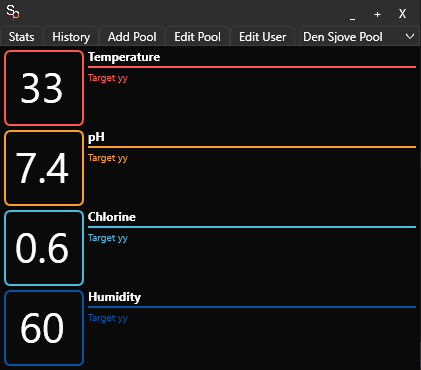
\includegraphics[width=0.5\linewidth]{figs/implementering/winstatview}
	\caption{WinStatView}
	\label{fig:winstatview}
\end{figure}

En controller oprettes, som kan hente de nuværende data. Når ViewDidLoad bliver kaldt på controlleren kalder den følgende funktion.
\lstset{style=sharpc}
\begin{lstlisting}
        public void DisplaySensorData(List<Tuple<SensorTypes, double>> sensorData)
        {
        	foreach (var sensor in sensorData)
        	{
        		switch (sensor.Item1)
        		{
        			case SensorTypes.Temperature:
        			TemperatureStatViewer.Parameter = string.Format($"{sensor.Item2}");
        			break;
        			case SensorTypes.Ph:
        			PhStatViewer.Parameter = string.Format($"{sensor.Item2}");
        			break;
        			case SensorTypes.Chlorine:
        			ChlorineStatViewer.Parameter = string.Format($"{sensor.Item2}");
        			break;
        			case SensorTypes.Humidity:
        			HumidityStatViewer.Parameter = string.Format($"{sensor.Item2}");
        			break;
        		} 
        	}
        }
\end{lstlisting}
Den korrekte StatViewer vælges og dens Parameter sættes til at være det nyeste data.

En StatViewer er en custom wpf control, som er lavet til dette formål. Den har en farve der repræsenterer sensor typen, og tekstfelter til property'en Parameter, hvori nuværende data er, Target værdi og sensor typen. 
På figur~\ref{fig:winstatview} ses fire StatViewers. En til hver sensor. 

StatViewer klassen er har givet fire ekstra properties. I koden nedenfor ses et eksempel.
\lstset{style=sharpc}
\begin{lstlisting}
public class StatViewer : Button
{
	public string Parameter
	{
		get { return (string)GetValue(ParameterProperty); }
		set { SetValue(ParameterProperty, value); }
	}
	
	public static readonly DependencyProperty ParameterProperty =
	DependencyProperty.RegisterAttached(
	"Parameter",
	typeof(string),
	typeof(StatViewer),
	new FrameworkPropertyMetadata("XX"));
	...
\end{lstlisting}
På denne måde er properties til BorderColor, Parameter og ParameterTarget. ParameterTarget er der, fordi det var planlagt at den skulle vise den ønskede værdi, men det er ikke implementeret.

Udseendet på StatViewer er defineret i en template der ligger i StatViewerTheme.xaml. Det er et ResourceDictionary, hvilket tillader at adskille Resourcer fra vinduerne i xaml.
Templaten ses nedenfor.
\lstset{style=sharpc}
\begin{lstlisting}
<!-- StatView template -->
<Style x:Key="{x:Type local:StatViewer}" TargetType="{x:Type local:StatViewer}">
<Setter Property="Foreground" Value="{StaticResource SpWhite}"/>
</Style>
<ControlTemplate x:Key="StatViewer" TargetType="local:StatViewer">
<Grid Height="80">
<Grid.ColumnDefinitions>
<ColumnDefinition Width="84"/>
<ColumnDefinition Width="*"/>
</Grid.ColumnDefinitions>
<Grid.RowDefinitions>
<RowDefinition Height="18"/>
<RowDefinition Height="6"/>
<RowDefinition Height="*"/>
<RowDefinition Height="22"/>
</Grid.RowDefinitions>
<Border Grid.Row="0" Grid.RowSpan="4" Grid.Column="0" Background="#00000000" Width="80" HorizontalAlignment="Left" BorderThickness="2" BorderBrush="{TemplateBinding BorderColor}" CornerRadius="5" Margin="4, 4, 0, 0"/>
<TextBlock Text="{TemplateBinding Content}" Grid.Row="0"  Grid.Column="1" HorizontalAlignment="Left" Foreground="{TemplateBinding Foreground}"  Margin="4,2,0,0" FontWeight="Bold" />
<Rectangle Grid.Row="1" Grid.Column="1" Height="2" Fill="{TemplateBinding BorderColor}" Margin="4, 0" />
<TextBlock Grid.Row="0" Grid.RowSpan="4" Grid.Column="0" Text="{TemplateBinding Parameter}" Foreground="{TemplateBinding Foreground}" HorizontalAlignment="Center" Margin="0,0,0,0" VerticalAlignment="Center" FontSize="42"/>
<TextBlock Grid.Row="2" Grid.Column="1" Text="{TemplateBinding ParameterTarget}" Foreground="{TemplateBinding BorderColor}" HorizontalAlignment="Left" VerticalAlignment="Top" Margin="4,0,0,0" FontSize="10"/>
</Grid>
</ControlTemplate>
\end{lstlisting}
Bemærk TargetType="local:StatViewer". Templaten er til StatViewer og de steder der står TemplateBinding forbindes de properties der var blevet tilføjet.